
The C++ standardization process is democratic. The committee is called WG21 (Working Group 21) and was formed in 1990-91. The officers of WG 21 are:

\begin{itemize}
\item 
Convener: chairs the WG21, sets the meeting schedule, and appoints Study Groups

\item 
Project Editor: applies changes to the working draft of the C++ standard

\item 
Secretary: assigns minutes of the WG21 meetings
\end{itemize}

The image shows you the various subgroups and Study Groups of the committee.

\begin{center}
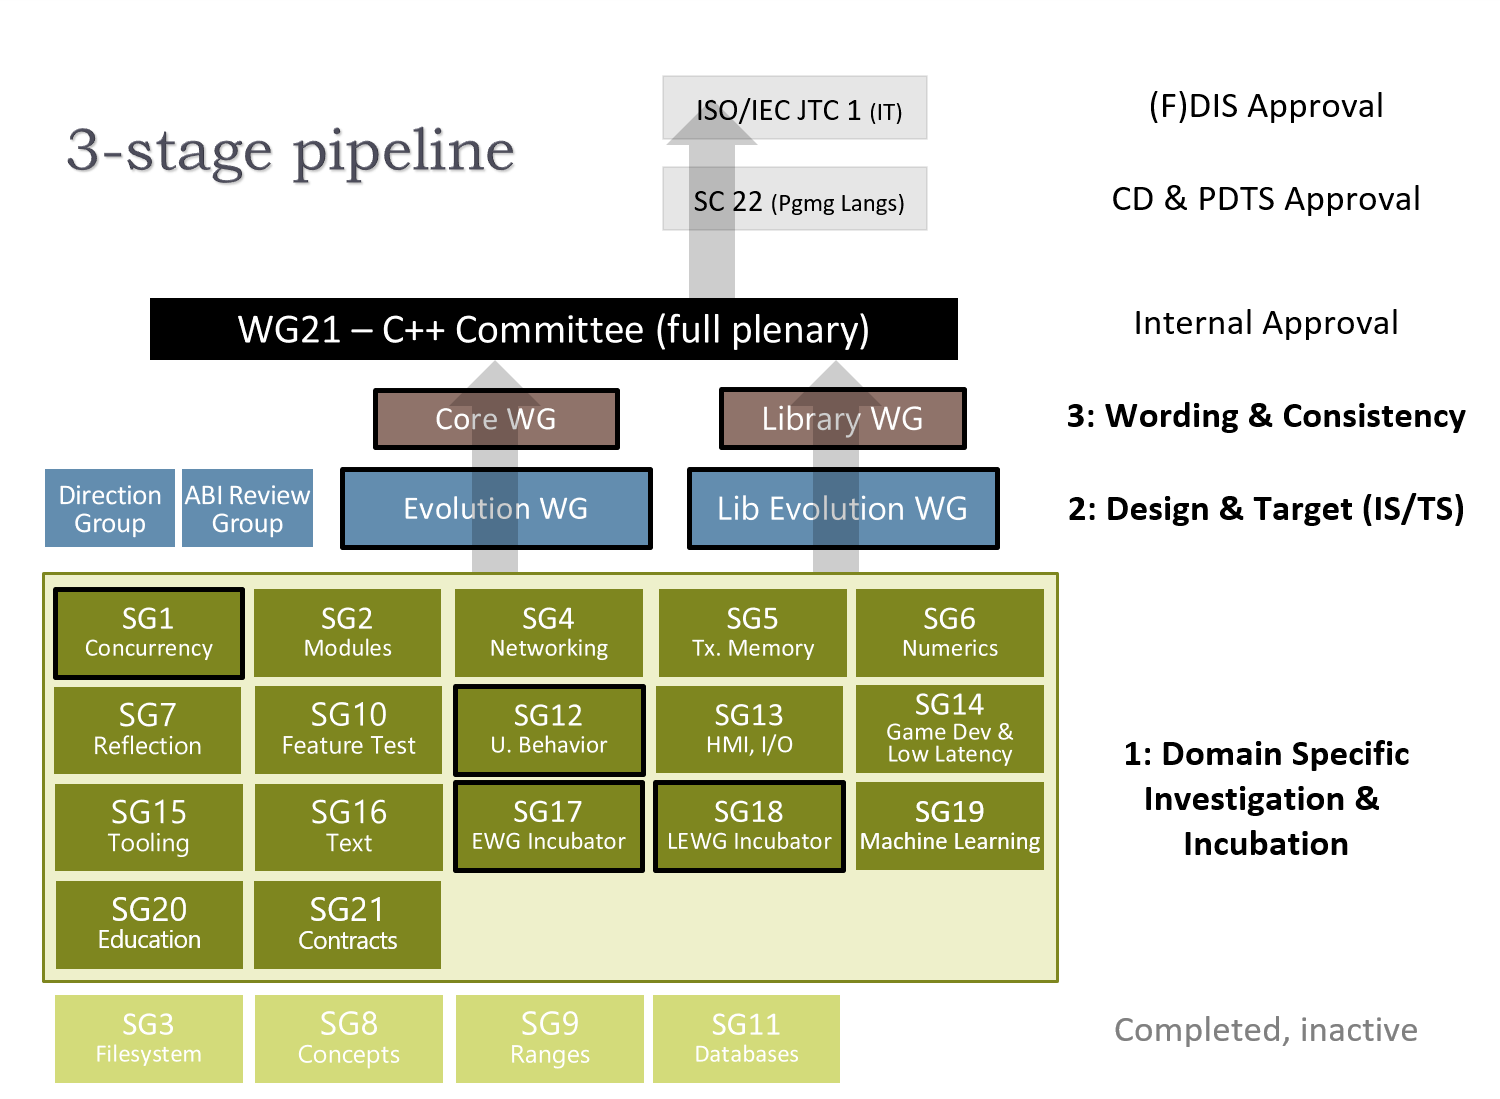
\includegraphics[width=1.0\textwidth]{content/1/chapter2/images/1.png}\\
Study groups in the C++ standardization process
\end{center}

The committee is organized into a three-stage pipeline consisting of several subgroups. SG stands for Study Group.